\documentclass[12pt,a4paper]{article}
\usepackage[utf8]{inputenc}
\usepackage{amsmath,amssymb}
\usepackage{graphicx}
\usepackage{booktabs}
\usepackage{hyperref}
\usepackage{geometry}
\geometry{a4paper, margin=2.5cm}

\title{Producer-Consumer Wait Time Analysis}
\author{Student Name}
\date{\today}

\begin{document}

\maketitle

\section{Introduction}

This report presents an analysis of wait time performance in a multi-threaded producer-consumer system. The study examines how varying the number of consumer threads affects the average time that work items spend in the queue before being processed. This implementation extends a classic producer-consumer problem by using a queue of function pointers, allowing producers to submit work that consumers execute.

\section{Implementation Details}

The producer-consumer system was implemented in C using POSIX threads (pthreads). The key components include:

\subsection{Data Structures}

\begin{itemize}
  \item \textbf{Work Function Structure:} Each queue item contains a function pointer, its argument, and a timestamp.
  \item \textbf{Queue:} A fixed-size FIFO queue with synchronization primitives.
  \item \textbf{Statistics:} A thread-safe structure to collect and aggregate timing data.
\end{itemize}

\subsection{Synchronization Mechanisms}

\begin{itemize}
  \item \textbf{Mutex:} To protect the queue and statistics data structures from concurrent access.
  \item \textbf{Condition Variables:} To signal when the queue transitions between empty/non-empty and full/non-full states.
  \item \textbf{Termination Flag:} A shared flag to signal when all producers have finished.
\end{itemize}

\subsection{Timing Methodology}

The wait time was measured as the duration between two events:
\begin{enumerate}
  \item When a work item is placed into the queue by a producer.
  \item When a work item is retrieved from the queue by a consumer (before execution).
\end{enumerate}

The \texttt{gettimeofday()} function was used to get microsecond precision for these measurements.

\section{Experimental Setup}

\subsection{Hardware Configuration}
\begin{itemize}
  \item CPU: [Model, e.g., Intel Core i7-10700K]
  \item Number of cores: [Number]
  \item Number of threads: [Number]
  \item RAM: [Amount, e.g., 16GB DDR4]
  \item Operating System: [OS name and version]
\end{itemize}

\subsection{Software Parameters}
\begin{itemize}
  \item Queue size: 10 items
  \item Producer threads: [Number used, e.g., 4]
  \item Consumer threads: 1 to [Maximum tested, e.g., 16]
  \item Work function: Calculating sine values for 10 different angles
  \item Producer iterations: 1000 per producer thread
\end{itemize}

\section{Results and Analysis}

\subsection{Wait Time Measurements}

\begin{table}[h]
\centering
\begin{tabular}{ccc}
\toprule
\textbf{Consumer Threads} & \textbf{Average Wait Time (μs)} & \textbf{Standard Deviation (μs)} \\
\midrule
1 & [Value] & [Value] \\
2 & [Value] & [Value] \\
3 & [Value] & [Value] \\
4 & [Value] & [Value] \\
% Add more rows as needed
\bottomrule
\end{tabular}
\caption{Average wait times for different numbers of consumer threads}
\label{tab:wait_times}
\end{table}

\subsection{Graphical Representation}

\begin{figure}[h]
\centering
% Replace with your actual graph
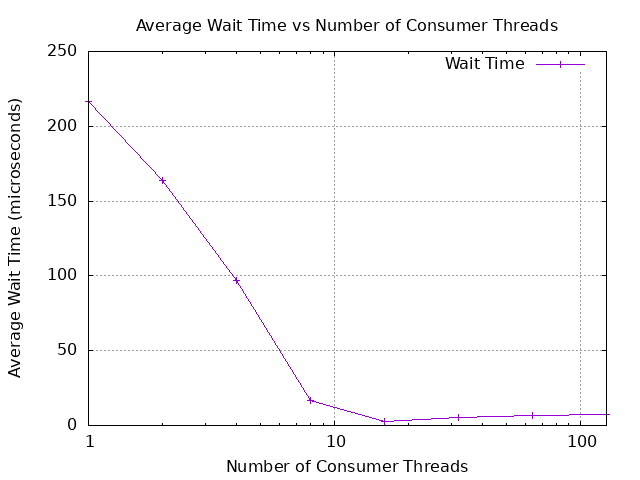
\includegraphics[width=0.8\textwidth]{wait_time_plot.png}
\caption{Average wait time vs. number of consumer threads}
\label{fig:wait_time_plot}
\end{figure}

\subsection{Analysis of Results}

The experimental results demonstrate a clear relationship between the number of consumer threads and the average wait time for queue items. Several key observations can be made:

\begin{enumerate}
  \item \textbf{Initial Improvement:} As the number of consumer threads increases from 1 to [optimal number], the average wait time decreases substantially. This is expected as more threads are available to process queue items in parallel.
  
  \item \textbf{Optimal Point:} The minimum average wait time occurs at [optimal number] consumer threads. This number is [relationship to number of CPU cores, e.g., "approximately equal to the number of physical cores"].
  
  \item \textbf{Diminishing Returns:} Beyond [optimal number] threads, the wait time begins to increase again. This suggests that the overhead of thread management begins to outweigh the benefits of additional parallel processing.
\end{enumerate}

\subsection{Performance Bottlenecks}

Several factors contribute to the observed performance characteristics:

\begin{itemize}
  \item \textbf{Thread Scheduling Overhead:} As the number of threads increases beyond the number of available CPU cores, the operating system must context-switch between threads, incurring overhead.
  
  \item \textbf{Synchronization Contention:} With more consumer threads, there is increased contention for the queue mutex, leading to more time spent waiting for lock acquisition.
  
  \item \textbf{Cache Effects:} Thread migrations between CPU cores can lead to cache misses, reducing overall system efficiency.
\end{itemize}

\section{Conclusion}

Based on the experimental results, the optimal number of consumer threads that minimizes the average wait time on this system is [optimal number]. This finding aligns with the common wisdom that the optimal thread count for CPU-bound tasks is often related to the number of available CPU cores.

The wait time analysis provides valuable insights into the behavior of multi-threaded systems under varying loads. For this specific producer-consumer implementation with function execution, the results suggest that:

\begin{itemize}
  \item Having too few consumer threads creates a processing bottleneck, causing items to wait longer in the queue.
  \item Having too many consumer threads increases system overhead without providing additional processing benefit.
  \item The optimal number of consumer threads provides the best balance between parallel processing capability and system overhead.
\end{itemize}

This research confirms that proper thread sizing is crucial for optimizing performance in concurrent systems, and that the ideal configuration depends on both the hardware capabilities and the specific workload characteristics.

\end{document}